\documentclass[10pt,a4paper]{article}
\usepackage[a4paper,margin=19mm]{geometry}
\usepackage[T1]{fontenc}
\usepackage{palatino}
\usepackage{xcolor}
\usepackage{hyperref}
\usepackage{enumitem}
\usepackage{tikz}
\usepackage[most]{tcolorbox}
\usetikzlibrary{positioning,arrows.meta}
\definecolor{navy}{HTML}{17365D}
\definecolor{bluegrey}{HTML}{EAF0F5}
\definecolor{ink}{HTML}{202A34}
\hypersetup{colorlinks=true,urlcolor=navy}
\setlength{\parindent}{0pt}
\setlist[itemize]{leftmargin=1.2em,noitemsep,topsep=2pt}
\newtcolorbox{summarybox}{colback=bluegrey,colframe=navy,boxrule=0pt,leftrule=2.4pt,arc=0pt,left=10pt,right=10pt,top=8pt,bottom=8pt}
\newtcolorbox{metricbox}[1]{colback=bluegrey,colframe=bluegrey,boxrule=0pt,arc=0pt,left=9pt,right=9pt,top=7pt,bottom=7pt,title={\color{navy}\footnotesize\bfseries #1},fonttitle=\bfseries}
\begin{document}
\color{ink}
\begin{tikzpicture}[remember picture,overlay]
\fill[navy] (current page.north west) rectangle ([yshift=-7mm]current page.north east);
\end{tikzpicture}
\vspace*{4mm}
{\LARGE\bfseries\color{navy} Remote Patient Monitoring System}\par
\vspace{3pt}
{\small Xuan Li Feng \quad\textbar\quad Imperial College London \quad\textbar\quad 2025}\par
\vspace{10pt}
\begin{summarybox}
\textbf{Public technical summary.} A desktop application for reviewing live physiological signals, patient records, and alerts through a structured, extensible clinical software architecture.
\end{summarybox}
\vspace{10pt}
\textbf{Engineering objective}\par\vspace{2pt}
How can a desktop system give clinicians a coherent view of multiple patients, live vital signs, abnormal events, and stored clinical information?\par
\vspace{11pt}
\textbf{System workflow}\par\vspace{5pt}
\begin{center}
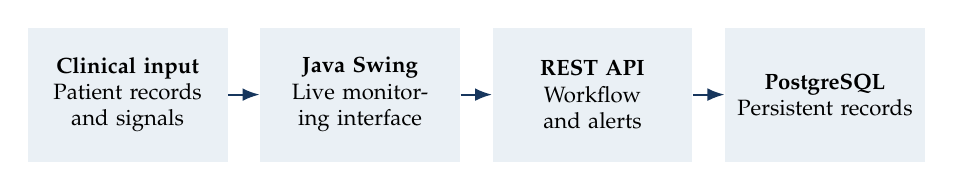
\begin{tikzpicture}[node distance=4mm and 4mm, every node/.style={align=center,font=\footnotesize}, flow/.style={-Latex,draw=navy,line width=.7pt}]
\node[fill=bluegrey,text width=.19\linewidth,minimum height=17mm] (a) {\textbf{Clinical input}\\Patient records and signals};
\node[fill=bluegrey,text width=.19\linewidth,minimum height=17mm,right=of a] (b) {\textbf{Java Swing}\\Live monitoring interface};
\node[fill=bluegrey,text width=.19\linewidth,minimum height=17mm,right=of b] (c) {\textbf{REST API}\\Workflow and alerts};
\node[fill=bluegrey,text width=.19\linewidth,minimum height=17mm,right=of c] (d) {\textbf{PostgreSQL}\\Persistent records};
\draw[flow] (a) -- (b); \draw[flow] (b) -- (c); \draw[flow] (c) -- (d);
\end{tikzpicture}
\end{center}
\vspace{7pt}
\begin{minipage}[t]{0.485\linewidth}
\textbf{Implemented functionality}\par\vspace{3pt}
\begin{itemize}
\item Multi-patient interface with live ECG and respiration waveform visualisation.
\item Patient onboarding, persistent clinical records, and historical review.
\item Visual and audio alerts with event acknowledgement and stored alert causes.
\end{itemize}
\end{minipage}\hfill
\begin{minipage}[t]{0.485\linewidth}
\textbf{System design}\par\vspace{3pt}
\begin{itemize}
\item Java Swing client connected to REST services and a PostgreSQL backend.
\item Digital Twin visualisation module designed as an extensible interface.
\item JUnit test suite and Gradle build workflow supporting quality control.
\end{itemize}
\end{minipage}
\vspace{10pt}
\textbf{Evidence at a glance}\par\vspace{5pt}
\begin{minipage}[t]{0.485\linewidth}
\begin{metricbox}{CLINICAL WORKFLOW}
{\Large\bfseries\color{navy} End to end}\par\vspace{2pt}
From patient onboarding to monitoring, alert acknowledgement, and record review.
\end{metricbox}
\end{minipage}\hfill
\begin{minipage}[t]{0.485\linewidth}
\begin{metricbox}{SYSTEM ARCHITECTURE}
{\Large\bfseries\color{navy} 3 layers}\par\vspace{2pt}
Presentation, application, and persistent data layers with clear responsibilities.
\end{metricbox}
\end{minipage}
\vspace{10pt}
\textbf{Project outcome}\par\vspace{3pt}
The completed prototype demonstrated a coherent clinical workflow and a modular software foundation for future monitoring and simulation features, without coupling the interface to one hardware device.
\vfill
\color{navy}\rule{\linewidth}{0.35pt}\par\vspace{4pt}
{\footnotesize\textbf{Technical tools}\quad Java \enspace Swing \enspace REST APIs \enspace PostgreSQL \enspace Gradle \enspace JUnit \enspace digital health software}
\end{document}
